\documentclass{article}
\usepackage{graphicx}

\title{%
\vspace{-2.5cm}
\textbf{Nintendo Entertainment System Emulator}\\
Project Vision and Scope
}
\date{\today}
\author{Kajetan Lach}

\begin{document}

\maketitle

\begin{figure}[h]
    \centering
    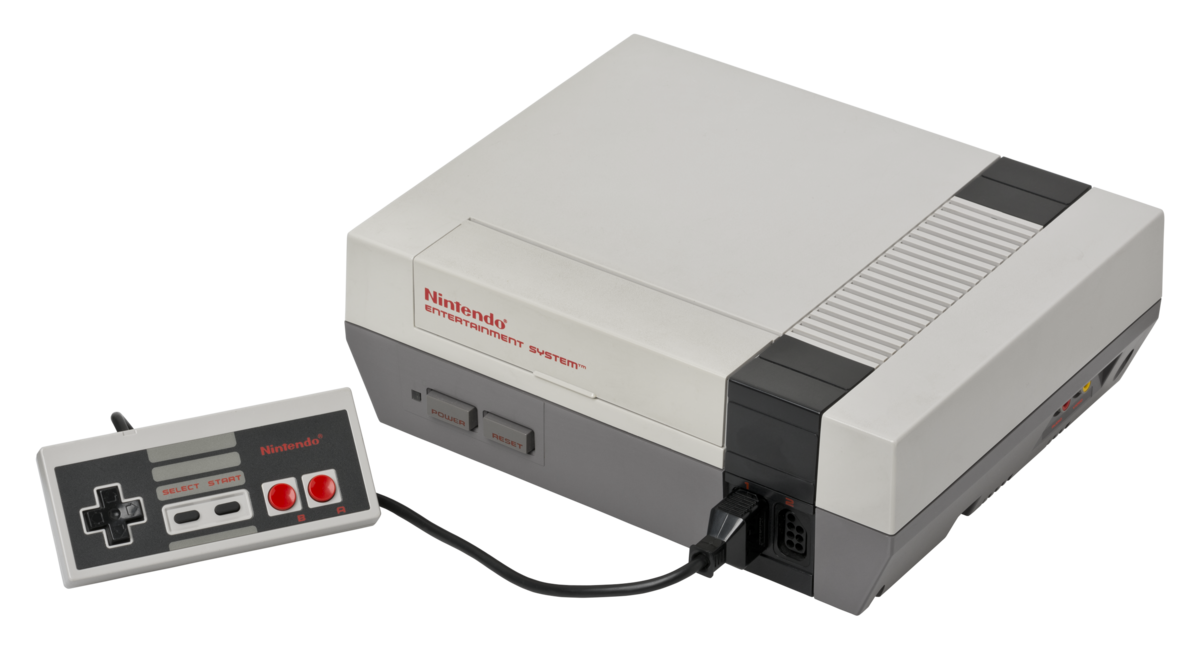
\includegraphics[width=0.7\textwidth]{NES.png}
\end{figure}

\section{Introduction}
Emulating old hardware can be an enjoyable and educational programming exercise. While being a project of non-trivial complexity, it's still relatively easy to grasp for a small team of young developers thanks to the simplicity of older computer architectures. Since emulating such systems requires an understanding of their inner workings, it's an excellent way to learn how computers operate at the lowest levels. Beyond its educational aspects, emulation software can be both useful and entertaining for users.

The \textbf{Nintendo Entertainment System (NES)} is an 8-bit home video game console released by Japanese video game company Nintendo in 1983. Regarded as one of the most influential consoles ever made, it helped revitalise the American gaming industry following the video game crash of 1983, pioneered a now-standard in video games industry business model of licensing third-party developers to produce and distribute games for platforms, and featured several groundbreaking games, such as \textit{Super Mario Bros} (1985), \textit{The Legend of Zelda} (1986), \textit{Metroid} (1986) and \textit{Mega Man} (1987), which became major franchises and pop-culture phenomenas.

\section{Vision statement}
The \textbf{NES Console Emulator} project aims to create a high-quality, user-friendly emulator that faithfully replicates the functionality of the Nintendo Entertainment System (NES), enabling users to experience retro gaming with accuracy and ease. The project is designed as an educational tool for deepening understanding of low-level computing and programming concepts for young developers, while also providing a functional application that brings classic NES games to modern hardware for its end users.
\subsection{Goals}
\textbf{Gain experience:} Develop a project that offers an in-depth learning experience in computer architecture and emulator development. Through emulation, one can gain familiarity with fundamental modern-computing concepts, such as memory management, processor instruction sets, systems architectures and graphical rendering in a manageable scope.

\noindent\textbf{Functional Usability:} Create an emulator that is easy to use and can reliably run the majority of NES ROMs, making it suitable for casual users and retro gaming enthusiasts.

\noindent\textbf{Accessibility:} Design both project's repository and interface in a way that enables code readability, straightforward usage and easy setup and gameplay, ensuring that users of all experience levels can enjoy this software.

\subsection{Objectives}
\textbf{Emulation accuracy:} Achieve high accuracy in the emulation of NES CPU (\textit{Central Processing Unit}), PPU (\textit{Picture Processing Unit}), and APU (\textit{Audio Processing Unit}), ensuring that most commercial NES ROMs are compatible and perform well within the emulator.

\noindent\textbf{User-Friendly GUI:} Design a basic, accessible graphical user interface that includes essential features such as ROM loading, game controls, and configuration options for graphics and audio.

\noindent\textbf{Performance Optimization:} Optimize the emulator to minimize resource consumption, allowing smooth gameplay even on lower-spec computers, while maintaining accuracy and stability.

\section{Target audience}
\textbf{Casual Gamers:} People interested in retro gaming as a casual activity, who seek a simple and accessible way to play NES games without needing specialized hardware.

\noindent\textbf{Retro Gaming Enthusiasts:} Individuals passionate about classic games who are looking for an accurate emulation experience that respects the authenticity of the original NES console.

\noindent\textbf{Speedrunners:} Competitive gamers focused on mastering specific games and achieving record-breaking times, who require precise emulation to practice and compete effectively.

\noindent\textbf{Archivists and Historians:} Individuals and organizations focused on preserving digital and cultural artifacts, using the emulator to maintain access to games that contribute to pop culture history and technology evolution.

\noindent\textbf{Developers:} Programmers interested in open source software, emulation development and both hardware and software fundamental concepts.

\section{Scope limitations and project boundaries}
\textbf{No Built-in Games:} The emulator will not include any pre-installed NES games due to copyright restrictions. Users will need to provide their own ROMs, ensuring compliance with legal standards and protecting intellectual property rights.

\noindent\textbf{No Save Systems:} The emulator will not feature any save system on it's own. The original NES didn't save games, and only some games that came out with internal memory would save user's progress. Those cases should be covered by the emulator.

\noindent\textbf{Limited Accuracy:} Achieving 100\% accuracy in emulating all NES games is not feasible within the scope of this project. While the goal is to ensure compatibility with a wide range of ROMs, some games may experience inaccuracies or bugs due to the inherent complexities of emulation.

\noindent\textbf{Minimal Customization Options:} The emulator will not include extensive customization features for graphics, controls, or audio settings. It will offer basic configuration options to enhance user experience but will not delve into advanced modding capabilities.

\noindent\textbf{No Hardware Integration:} There will be no support for physical peripherals such as original NES controllers or other hardware accessories. The emulator will function solely as a software application, designed to work with standard PC input devices.

\noindent\textbf{Limited Debugging and Development Tools:} The project will not provide built-in debugging or development tools for users interested in creating or modifying games. The focus will be on end-user experience rather than game development support.



\end{document}
